% Task 1: Chinese translation of the user-provided Zhang calibration paper.
% Integration Worker owns this file. Chapter content belongs in sections/*.tex.
% Use the TeX Live bundled CJK fonts for reproducible compilation on macOS
% installations where ctex's default STHeiti face is not registered.
\documentclass[UTF8,a4paper,10pt,fontset=fandol]{ctexart}

% ---- Global document configuration (the only global configuration source) ----
\usepackage[a4paper,left=2.0cm,right=2.0cm,top=2.0cm,bottom=2.0cm]{geometry}
\usepackage{amsmath,amssymb,bm}
\usepackage{array,booktabs}
\usepackage{graphicx}
\usepackage{caption}
\usepackage{enumitem}
\usepackage{xcolor}
\usepackage[hidelinks]{hyperref}
\usepackage{url}

\graphicspath{{figures/}}
\setlength{\parindent}{2em}
\setlength{\parskip}{0.25em}
\linespread{1.05}
\captionsetup{font=small,labelfont=bf}
\setlist{nosep}

% Shared notation macros. Chapter workers should use these where applicable.
\newcommand{\vect}[1]{\boldsymbol{#1}}
\newcommand{\mat}[1]{\mathbf{#1}}
\newcommand{\T}{\mathsf{T}}
\newcommand{\R}{\mathbb{R}}
\newcommand{\norm}[1]{\left\lVert#1\right\rVert}
\newcommand{\keywords}[1]{\par\noindent\textbf{关键词：}#1}

\hypersetup{
  pdftitle={通过从未知方向观察平面实现灵活的相机标定},
  pdfauthor={课程作业译稿},
  pdfsubject={张正友标定法论文中文翻译}
}

\title{\heiti 通过从未知方向观察平面实现灵活的相机标定}
\author{课程作业译稿\\[-0.25em]\small 原论文作者：Zhengyou Zhang}
\date{}

\begin{document}
\maketitle

% Keep the paper's original section order. Each chapter is maintained by a
% separate translation worker; do not place substantive prose in this file.
\begin{abstract}
本文提出一种灵活的新技术，用于方便地完成相机标定。该方法仅要求相机在少数（至少两个）不同方向下观测一个平面模板。相机或平面模板均可自由移动，且不需要知道其运动。方法对镜头的径向畸变进行建模。所提出的过程由一个闭式解开始，随后依据最大似然准则进行非线性细化。我们使用计算机仿真数据和真实数据对所提出的技术进行了测试，并获得了非常好的结果。与使用昂贵设备（例如两个或三个相互正交的平面）的传统技术相比，所提出的技术易于使用且具有灵活性。它使三维计算机视觉从实验室环境向现实应用迈进一步。相应的软件可从作者的网页获得。
\end{abstract}
\keywords{相机标定；内参数；镜头畸变；基于平面的灵活标定；运动分析；模型获取}

\section{动机}

相机标定是三维计算机视觉中从二维图像提取度量信息的必要步骤。该领域已经开展了大量工作，起初来自摄影测量学界（例如见文献~\cite{brown1971close,faig1975calibration}），近来则更多来自计算机视觉领域（例如见文献~\cite{gennery1979stereo,ganapathy1984decomposition,tsai1987versatile,faugeras1986stereo,weng1992camera,wei1993complete,maybank1992theory,faugeras1992self,triggs1998autocalibration}）。粗略地说，我们可以将这些技术分为两类：

\textbf{摄影测量标定。} 标定通过观测一个标定物体来完成，该物体在三维空间中的几何形状已知且具有很高的精度。标定可以非常高效地完成~\cite{faugeras1993three}。标定物体通常由两个或三个彼此正交的平面组成。有时也使用一个经历精确已知平移的平面~\cite{tsai1987versatile}。这些方法需要昂贵的标定装置和复杂的设置。

\textbf{自标定。} 这类技术不使用任何标定物体。仅通过在静态场景中移动相机，场景的刚性通常就可以利用纯图像信息，从一次相机位移中为相机的内参数提供两个约束~\cite{maybank1992theory}。因此，如果图像由同一台具有固定内参数的相机拍摄，那么三幅图像之间的对应关系就足以恢复内参数和外参数，并据此在相似变换意义下重建三维结构~\cite{luong1997self,hartley1994several}。尽管这种方法非常灵活，但目前还不够成熟~\cite{bougnoux1998projective}。由于需要估计的参数很多，我们无法始终获得可靠的结果。

还存在其他技术，例如利用正交方向的消失点进行标定~\cite{caprile1990vanishing,liebowitz1998metric}，以及利用纯旋转进行标定~\cite{hartley1994rotating,stein1995accurate}。

我们当前的研究聚焦于桌面视觉系统（desktop vision system，DVS），因为使用 DVS 的潜力很大。相机正变得廉价且无处不在。DVS 面向普通大众，而他们并非计算机视觉专家。典型的计算机用户只会偶尔执行视觉任务，因此不愿意为昂贵的设备投资。因此，灵活性、鲁棒性和低成本十分重要。本文所述的相机标定技术正是在这些考虑下开发的。

所提出的技术仅要求相机在少数（至少两个）不同方向下观测一个平面模板。该模板可以用激光打印机打印出来，并附着在一个“合理的”平面表面上（例如硬质书封面）。相机或平面模板均可用手移动，且不需要知道其运动。所提出的方法介于摄影测量标定和自标定之间，这是因为我们使用的是二维度量信息，而不是三维度量信息或纯粹的隐式信息。我们使用计算机仿真数据和真实数据对所提出的技术进行了测试，并获得了非常好的结果。与传统方法相比，所提出的技术灵活得多；与自标定相比，它具有相当程度的鲁棒性。我们相信，这项新技术使三维计算机视觉从实验室环境向现实世界迈进一步。

值得注意的是，Bill Triggs~\cite{triggs1998autocalibration} 最近提出了一种自标定技术，它至少需要对平面场景进行五次观测。该技术比我们的方法更加灵活，但存在初始化困难。Liebowitz 和 Zisserman~\cite{liebowitz1998metric} 描述了一种针对平面透视图像的度量校正技术，所使用的度量信息包括一个已知角度、两个相等但未知的角度以及一个已知长度比。他们还提到，只要存在这样的度量校正平面，就可以对相机的内参数进行标定，尽管他们没有给出算法或实验结果。

本文的组织结构如下。第 2 节描述从观测单个平面得到的基本约束。第 3 节描述标定过程：我们先给出一个闭式解，然后进行非线性优化，同时对镜头径向畸变进行建模。第 4 节研究所提出的相机标定技术失效的配置；在实践中，这些情况很容易避免。第 5 节给出实验结果，并使用计算机仿真数据和真实数据验证所提出的技术。附录给出若干细节，包括估计模型平面与其图像之间单应性的技术。

\section{基本方程}

我们研究通过观测单个平面得到的相机内参数约束。首先介绍本文使用的记号。

\subsection{记号}

二维点记为
$\mathbf m=[u,v]^{\T}$，三维点记为
$\mathbf M=[X,Y,Z]^{\T}$。我们用波浪号表示在向量末尾添加 1 后得到的增广向量，即
$\widetilde{\mathbf m}=[u,v,1]^{\T}$，以及
$\widetilde{\mathbf M}=[X,Y,Z,1]^{\T}$。相机采用通常的针孔模型：三维点 $\mathbf M$ 与其图像投影 $\mathbf m$ 之间的关系为
\begin{equation}
    s\widetilde{\mathbf m}=\mathbf A
    \begin{bmatrix}\mathbf R & \mathbf t\end{bmatrix}
    \widetilde{\mathbf M},
    \qquad
    \mathbf A=\begin{bmatrix}
        \alpha & c & u_0\\
        0 & \beta & v_0\\
        0 & 0 & 1
    \end{bmatrix}.
    \label{eq:pinhole}
\end{equation}
其中，$s$ 是任意尺度因子；$(\mathbf R,\mathbf t)$ 称为外参数，分别是联系世界坐标系与相机坐标系的旋转和平移；$\mathbf A$ 称为相机内参数矩阵；$(u_0,v_0)$ 是主点的坐标；$\alpha$ 和 $\beta$ 分别是图像 $u$ 轴和 $v$ 轴方向的尺度因子；$c$ 是两个图像轴之间的倾斜参数。

我们使用如下记号缩写：
$\mathbf A^{-\T}$ 表示 $(\mathbf A^{-1})^{\T}$ 或 $(\mathbf A^{\T})^{-1}$。

\subsection{模型平面与其图像之间的单应性}

不失一般性，假设模型平面位于世界坐标系的 $Z=0$ 平面上。将旋转矩阵 $\mathbf R$ 的第 $i$ 列记为 $\mathbf r_i$。由式~\eqref{eq:pinhole} 可得
\begin{equation*}
    s\begin{bmatrix}u\\v\\1\end{bmatrix}
    =\mathbf A
    \begin{bmatrix}\mathbf r_1 & \mathbf r_2 & \mathbf r_3 & \mathbf t\end{bmatrix}
    \begin{bmatrix}X\\Y\\0\\1\end{bmatrix}
    =\mathbf A
    \begin{bmatrix}\mathbf r_1 & \mathbf r_2 & \mathbf t\end{bmatrix}
    \begin{bmatrix}X\\Y\\1\end{bmatrix}.
\end{equation*}
虽然存在记号上的不严格之处，我们仍用 $\mathbf M$ 表示模型平面上的一个点，但此时 $\mathbf M=[X,Y]^{\T}$，因为 $Z$ 始终等于 0。相应地，$\widetilde{\mathbf M}=[X,Y,1]^{\T}$。因此，模型点 $\mathbf M$ 与其图像点 $\mathbf m$ 通过单应性矩阵 $\mathbf H$ 联系起来：
\begin{equation}
    s\widetilde{\mathbf m}=\mathbf H\widetilde{\mathbf M},
    \qquad
    \mathbf H=\mathbf A
    \begin{bmatrix}\mathbf r_1 & \mathbf r_2 & \mathbf t\end{bmatrix}.
    \label{eq:homography}
\end{equation}
显然，$3\times3$ 矩阵 $\mathbf H$ 只定义到一个尺度因子。

\subsection{内参数约束}

给定模型平面的一幅图像，即可估计一个单应性（见附录 A）。记该单应性为
$\mathbf H=\begin{bmatrix}\mathbf h_1&\mathbf h_2&\mathbf h_3\end{bmatrix}$。由式~\eqref{eq:homography} 可得
\begin{equation*}
    \begin{bmatrix}\mathbf h_1&\mathbf h_2&\mathbf h_3\end{bmatrix}
    =\lambda\mathbf A
    \begin{bmatrix}\mathbf r_1&\mathbf r_2&\mathbf t\end{bmatrix},
\end{equation*}
其中 $\lambda$ 是任意标量。利用 $\mathbf r_1$ 和 $\mathbf r_2$ 相互正交且均为单位向量这一事实，有
\begin{equation}
    \mathbf h_1^{\T}\mathbf A^{-\T}\mathbf A^{-1}\mathbf h_2=0.
    \label{eq:orthogonality}
\end{equation}
\begin{equation}
    \mathbf h_1^{\T}\mathbf A^{-\T}\mathbf A^{-1}\mathbf h_1
    =\mathbf h_2^{\T}\mathbf A^{-\T}\mathbf A^{-1}\mathbf h_2.
    \label{eq:equal-norm}
\end{equation}
这就是给定一个单应性时关于内参数的两个基本约束。由于一个单应性具有 8 个自由度，而外参数有 6 个（旋转 3 个、平移 3 个），因此我们只能得到关于内参数的 2 个约束。

% Translation worker B: Section 3 of the source paper.
\section{相机标定求解}\label{sec:calibration-solution}

本节详细介绍如何有效求解相机标定问题。首先给出解析解，随后介绍一种基于最大似然准则的非线性优化技术。最后考虑镜头畸变，从而给出解析解和非线性解。

\subsection{闭式解}\label{subsec:closed-form}

令
\begin{equation}
\begin{aligned}
\mat{B} &= \mat{A}^{-\T}\mat{A}^{-1}
\equiv
\begin{bmatrix}
B_{11} & B_{12} & B_{13}\\
B_{12} & B_{22} & B_{23}\\
B_{13} & B_{23} & B_{33}
\end{bmatrix}\\
&=
\begin{bmatrix}
\dfrac{1}{\alpha^2}
&-\dfrac{c}{\alpha^2\beta}
&\dfrac{cv_0-u_0\beta}{\alpha^2\beta}\\[0.6em]
-\dfrac{c}{\alpha^2\beta}
&\dfrac{c^2}{\alpha^2\beta^2}+\dfrac{1}{\beta^2}
&-\dfrac{c(cv_0-u_0\beta)}{\alpha^2\beta^2}-\dfrac{v_0}{\beta^2}\\[0.6em]
\dfrac{cv_0-u_0\beta}{\alpha^2\beta}
&-\dfrac{c(cv_0-u_0\beta)}{\alpha^2\beta^2}-\dfrac{v_0}{\beta^2}
&\dfrac{(cv_0-u_0\beta)^2}{\alpha^2\beta^2}+\dfrac{v_0^2}{\beta^2}+1
\end{bmatrix} .
\end{aligned}
\label{eq:intrinsic-constraint-matrix}
\end{equation}
注意，$\mat{B}$ 是对称矩阵，可以由一个六维向量定义：
\begin{equation}
\vect{b}=\left[B_{11},B_{12},B_{22},B_{13},B_{23},B_{33}\right]^{\T} .
\label{eq:intrinsic-constraint-vector}
\end{equation}
（实际上，它描述了绝对二次曲线在图像中的表示。）

设 $\mat{H}$ 的第 $i$ 个列向量为
\begin{equation*}
\vect{h}_i=\left[h_{i1},h_{i2},h_{i3}\right]^{\T} .
\end{equation*}
则有
\begin{equation}
\vect{h}_i^{\T}\mat{B}\vect{h}_j=\vect{v}_{ij}^{\T}\vect{b},
\label{eq:homography-constraint-vector}
\end{equation}
其中
\begin{equation*}
\vect{v}_{ij}=\left[
h_{i1}h_{j1},\;
h_{i1}h_{j2}+h_{i2}h_{j1},\;
h_{i2}h_{j2},\;
h_{i3}h_{j1}+h_{i1}h_{j3},\;
h_{i3}h_{j2}+h_{i2}h_{j3},\;
h_{i3}h_{j3}
\right]^{\T} .
\end{equation*}

因此，由给定单应性得到的两个基本约束（式~\eqref{eq:orthogonality} 和式~\eqref{eq:equal-norm}）可以改写为关于 $\vect{b}$ 的两个齐次方程：
\begin{equation}
\begin{bmatrix}
\vect{v}_{12}^{\T}\\
(\vect{v}_{11}-\vect{v}_{22})^{\T}
\end{bmatrix}\vect{b}=\vect{0} .
\label{eq:stacked-homography-constraints}
\end{equation}
如果观测到模型平面的 $n$ 幅图像，将 $n$ 组如式~\eqref{eq:stacked-homography-constraints} 所示的方程叠加，可得
\begin{equation}
\mat{V}\vect{b}=\vect{0},
\label{eq:calibration-linear-system}
\end{equation}
其中，$\mat{V}$ 是一个 $2n\times6$ 矩阵。当 $n\geq3$ 时，通常可以得到一个除尺度因子外唯一确定的解 $\vect{b}$。当 $n=2$ 时，可以施加无倾斜约束 $c=0$，即
\begin{equation*}
\left[0,1,0,0,0,0\right]\vect{b}=0,
\end{equation*}
并将其作为附加方程加入式~\eqref{eq:calibration-linear-system}。式~\eqref{eq:calibration-linear-system} 的解是与 $\mat{V}^{\T}\mat{V}$ 的最小特征值对应的特征向量（等价地，是与 $\mat{V}$ 的最小奇异值对应的右奇异向量）。

得到 $\vect{b}$ 后，即可计算相机内参数矩阵 $\mat{A}$；具体细节见附录~B。已知 $\mat{A}$ 后，每幅图像的外参数也可直接计算。由式~\eqref{eq:homography} 有
\begin{equation*}
\vect{r}_1=\lambda\mat{A}^{-1}\vect{h}_1,\qquad
\vect{r}_2=\lambda\mat{A}^{-1}\vect{h}_2,\qquad
\vect{r}_3=\vect{r}_1\times\vect{r}_2,\qquad
\vect{t}=\lambda\mat{A}^{-1}\vect{h}_3,
\end{equation*}
其中
\begin{equation*}
\lambda=\frac{1}{\norm{\mat{A}^{-1}\vect{h}_1}}
=\frac{1}{\norm{\mat{A}^{-1}\vect{h}_2}} .
\end{equation*}
当然，由于数据中存在噪声，按此方式计算得到的矩阵
 $\mat{R}=\left[\vect{r}_1,\vect{r}_2,\vect{r}_3\right]$
通常不满足旋转矩阵的性质。附录~C 描述了如何从一般的 $3\times3$ 矩阵估计最佳旋转矩阵的方法。

\subsection{最大似然估计}\label{subsec:maximum-likelihood}

上述解是通过最小化一个不具有物理意义的代数距离得到的。可以利用最大似然估计对其进行细化。

设给定模型平面的 $n$ 幅图像，模型平面上有 $m$ 个点。假设图像点受到独立同分布噪声的干扰。最大似然估计可以通过最小化下述泛函得到：
\begin{equation}
\sum_{i=1}^{n}\sum_{j=1}^{m}
\norm{m_{ij}-\widehat{m}(\mat{A},\mat{R}_i,\vect{t}_i,M_j)}^2 .
\label{eq:maximum-likelihood}
\end{equation}
其中，$\widehat{m}(\mat{A},\mat{R}_i,\vect{t}_i,M_j)$ 是根据式~\eqref{eq:homography} 将点 $M_j$ 投影到第 $i$ 幅图像上的结果。旋转 $\mat{R}$ 由一个三参数向量（记为 $\vect{r}$）参数化，该向量与旋转轴平行，其模长等于旋转角。$\mat{R}$ 与 $\vect{r}$ 通过 Rodrigues 公式相关联~\cite{faugeras1993three}。最小化式~\eqref{eq:maximum-likelihood} 是一个非线性最小化问题，使用 Minpack 中实现的 Levenberg--Marquardt 算法求解~\cite{more1977levenberg}。该算法需要 $\mat{A}$ 以及 $\{\mat{R}_i,\vect{t}_i\mid i=1..n\}$ 的初始估计，这些初始值可以通过上一小节所述的技术得到。

\subsection{处理径向畸变}\label{subsec:radial-distortion}

到目前为止，我们还没有考虑相机的镜头畸变。然而，桌面相机通常表现出显著的镜头畸变，尤其是径向畸变。本节仅考虑径向畸变的前两项。关于更复杂的模型，读者可参阅文献~\cite{slama1980manual,brown1971close,faig1975calibration,weng1992camera}。根据已有文献的报告~\cite{brown1971close,tsai1987versatile,wei1994implicit}，畸变函数很可能完全由径向分量主导，尤其由第一项主导。已有研究还发现，更复杂的建模不仅没有帮助（与传感器量化相比其影响可以忽略），还会导致数值不稳定~\cite{tsai1987versatile,wei1994implicit}。

令 $(u,v)$ 表示理想的（不可观测的、无畸变的）像素图像坐标，$(\breve{u},\breve{v})$ 表示与之对应的实际观测图像坐标。类似地，$(x,y)$ 和 $(\breve{x},\breve{y})$ 分别表示理想的（无畸变的）和实际的（有畸变的）归一化图像坐标。有如下关系~\cite{brown1971close,wei1994implicit}
\begin{align*}
\breve{x}&=x+x\left[k_1(x^2+y^2)+k_2(x^2+y^2)^2\right],\\
\breve{y}&=y+y\left[k_1(x^2+y^2)+k_2(x^2+y^2)^2\right],
\end{align*}
其中，$k_1$ 和 $k_2$ 是径向畸变系数。径向畸变的中心与主点相同。由
\begin{equation*}
\breve{u}=u_0+\alpha\breve{x}+c\breve{y},\qquad
\breve{v}=v_0+\beta\breve{y}
\end{equation*}
可得
\begin{align}
\breve{u}&=u+(u-u_0)\left[k_1(x^2+y^2)+k_2(x^2+y^2)^2\right],
\label{eq:radial-distortion-u}\\
\breve{v}&=v+(v-v_0)\left[k_1(x^2+y^2)+k_2(x^2+y^2)^2\right].
\label{eq:radial-distortion-v}
\end{align}

\paragraph{通过交替估计径向畸变。}
由于径向畸变预计较小，因此可以预期，使用第~\ref{subsec:maximum-likelihood} 节所述技术、简单地忽略畸变，也能够较为合理地估计其他五个内参数。一种策略是在估计其他参数之后再估计 $k_1$ 和 $k_2$。由式~\eqref{eq:radial-distortion-u} 和式~\eqref{eq:radial-distortion-v}，每幅图像中的每个点均可得到两个方程：
\begin{equation*}
\begin{bmatrix}
(u-u_0)(x^2+y^2) & (u-u_0)(x^2+y^2)^2\\
(v-v_0)(x^2+y^2) & (v-v_0)(x^2+y^2)^2
\end{bmatrix}
\begin{bmatrix}k_1\\k_2\end{bmatrix}
=
\begin{bmatrix}\breve{u}-u\\\breve{v}-v\end{bmatrix} .
\end{equation*}
给定 $n$ 幅图像中的 $m$ 个点，将所有方程叠加后总共得到 $2mn$ 个方程，或写成矩阵形式 $\mat{D}k=d$，其中 $k=[k_1,k_2]^{\T}$。线性最小二乘解为
\begin{equation}
k=(\mat{D}^{\T}\mat{D})^{-1}\mat{D}^{\T}d .
\label{eq:radial-linear-least-squares}
\end{equation}
得到 $k_1$ 和 $k_2$ 后，可以通过求解式~\eqref{eq:maximum-likelihood} 来细化其他参数，只需将其中的 $\widehat{m}(\mat{A},\mat{R}_i,\vect{t}_i,M_j)$ 替换为式~\eqref{eq:radial-distortion-u} 和式~\eqref{eq:radial-distortion-v} 所描述的投影。可以交替执行这两个过程，直到收敛。

\paragraph{完整的最大似然估计。}
通过实验发现，上述交替技术的收敛速度较慢。因此，对式~\eqref{eq:maximum-likelihood} 的自然扩展是通过最小化下述泛函来估计完整的参数集：
\begin{equation}
\sum_{i=1}^{n}\sum_{j=1}^{m}
\norm{m_{ij}-\breve{m}(\mat{A},k_1,k_2,\mat{R}_i,\vect{t}_i,M_j)}^2 .
\label{eq:complete-maximum-likelihood}
\end{equation}
其中，$\breve{m}(\mat{A},k_1,k_2,\mat{R}_i,\vect{t}_i,M_j)$ 是根据式~\eqref{eq:homography} 将点 $M_j$ 投影到第 $i$ 幅图像上、再依据式~\eqref{eq:radial-distortion-u} 和式~\eqref{eq:radial-distortion-v} 施加畸变后的结果。这是一个非线性最小化问题，使用 Minpack 中实现的 Levenberg--Marquardt 算法求解~\cite{more1977levenberg}。旋转仍然像第~\ref{subsec:maximum-likelihood} 节中一样由三维向量 $\vect{r}$ 参数化。$\mat{A}$ 以及 $\{\mat{R}_i,\vect{t}_i\mid i=1..n\}$ 的初始估计可以使用第~\ref{subsec:closed-form} 节或第~\ref{subsec:maximum-likelihood} 节所述技术获得。$k_1$ 和 $k_2$ 的初始估计可以使用上一段所述技术获得，也可以直接将其设为 $0$。

\subsection{总结}\label{subsec:calibration-summary}

推荐的相机标定流程如下：
\begin{enumerate}
    \item 打印一个模板，并将其粘贴到平面表面上；
    \item 通过移动平面或相机，在不同方向下拍摄几幅模型平面的图像；
    \item 检测图像中的特征点；
    \item 使用第~\ref{subsec:closed-form} 节所述的闭式解，估计五个内参数和全部外参数；
    \item 求解线性最小二乘问题~\eqref{eq:radial-linear-least-squares}，估计径向畸变系数；
    \item 通过最小化式~\eqref{eq:complete-maximum-likelihood} 对全部参数进行细化。
\end{enumerate}

% Translation worker B: Section 4 of the source paper.
\section{退化配置}\label{sec:degenerate-configurations}

本节研究这样一些配置：在这些配置中，增加图像并不会为相机内参数提供更多约束。由于式~\eqref{eq:orthogonality} 和式~\eqref{eq:equal-norm} 源自旋转矩阵的性质，如果 $\mat{R}_2$ 不独立于 $\mat{R}_1$，则第 2 幅图像不会提供额外约束。特别地，如果一个平面仅发生平移，则 $\mat{R}_2=\mat{R}_1$，此时第 2 幅图像对相机标定没有帮助。下面考虑一种更复杂的配置。

\noindent\textbf{命题 1.}
如果模型平面在第二个位置与其第一个位置平行，则第二个单应性不会提供额外约束。

证明因篇幅所限略去，可参见我们的技术报告~\cite{zhang1998flexible}。在实践中，退化配置非常容易避免：只需改变模型平面在相邻两次拍摄之间的方向即可。

% Section 5 translation from the user-provided paper.
\section{实验结果}\label{sec:experimental-results}

所提出的算法在计算机模拟数据和真实数据上都进行了测试。闭式解涉及对一个小型 \(2n\times 6\) 矩阵进行奇异值分解，其中 \(n\) 为图像数量。Levenberg--Marquardt 算法中的非线性细化经过 \(3\) 至 \(5\) 次迭代即可收敛。

\subsection{计算机模拟}\label{subsec:computer-simulations}

模拟相机的参数为
\(\alpha=1250\)、\(\beta=900\)、\(c=1.09083\)（等价于 \(89.95^\circ\)）、\(u_0=255\) 和 \(v_0=255\)。图像分辨率为 \(512\times512\)。模型平面是一个包含 \(10\times14=140\) 个角点的棋盘格（因此 \(v\) 方向的数据通常多于 \(u\) 方向），模板尺寸为 \(18\mathrm{cm}\times25\mathrm{cm}\)。平面的姿态用三维向量 \(\mathbf r\) 表示：\(\mathbf r\) 与旋转轴平行，其模等于旋转角。平面的位置用三维向量 \(\mathbf t\) 表示，单位为厘米。

\paragraph{噪声水平的影响}

在该实验中，使用三个平面，其姿态和位置分别为
\begin{equation}
\begin{aligned}
\mathbf r_1&=[20^\circ,0,0]^{\mathsf T},&
\mathbf t_1&=[-9,-12.5,500]^{\mathsf T},\\
\mathbf r_2&=[0,20^\circ,0]^{\mathsf T},&
\mathbf t_2&=[-9,-12.5,510]^{\mathsf T},\\
\mathbf r_3&=\frac{1}{\sqrt{5}}[-30^\circ,-30^\circ,-15^\circ]^{\mathsf T},&
\mathbf t_3&=[-10.5,-12.5,525]^{\mathsf T}.
\end{aligned}
\label{eq:simulation-poses}
\end{equation}
在投影得到的图像点上加入均值为 \(0\)、标准差为 \(\sigma\) 的高斯噪声。将估计得到的相机参数与真实值进行比较：对 \(\alpha\) 和 \(\beta\) 测量相对误差，对 \(u_0\) 和 \(v_0\) 测量绝对误差。噪声水平从 \(0.1\) 像素变化到 \(1.5\) 像素；对每个噪声水平进行 \(100\) 次相互独立的试验，图中结果取平均值。

\begin{figure}[htbp]
    \centering
    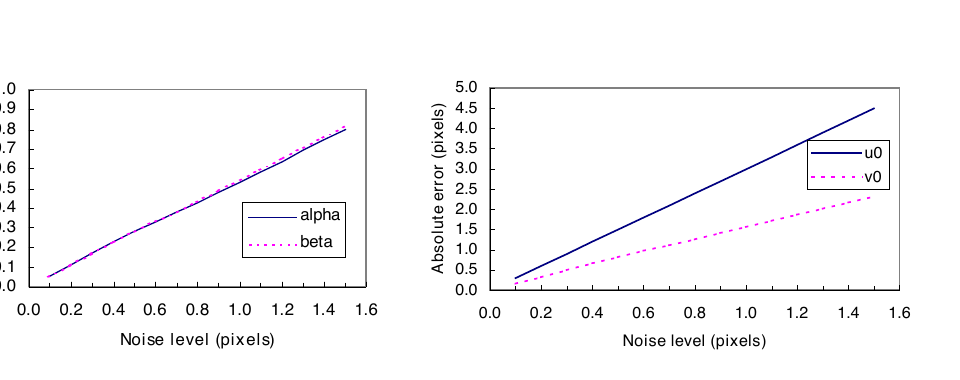
\includegraphics[width=0.88\linewidth]{figure1_noise_errors}
    \caption{图像点噪声水平对应的误差。}
    \label{fig:simulation-noise}
\end{figure}

如图\ref{fig:simulation-noise}所示，误差随噪声水平近似线性增加。参数 \(c\) 的误差未在图中给出，但具有相同的变化规律。当 \(\sigma=0.5\)（该噪声水平高于实际标定中的通常噪声）时，\(\alpha\) 和 \(\beta\) 的误差小于 \(0.3\%\)，而 \(u_0\) 和 \(v_0\) 的误差约为 \(1\) 像素。\(u_0\) 的误差大于 \(v_0\) 的误差，主要原因是 \(u\) 方向的数据少于 \(v\) 方向的数据。

\paragraph{模型平面图像数量的影响}

该实验考察图像数量（更准确地说，是模型平面图像的数量）对性能的影响。前 \(3\) 幅图像中模型平面的姿态和位置与上一小节相同。从第 \(4\) 幅图像开始，首先从均匀球面上随机选择旋转轴，然后施加 \(30^\circ\) 的旋转角。图像数量从 \(2\) 幅变化到 \(16\) 幅。对于每一个图像数量，进行 \(100\) 次相互独立的试验；除前 \(3\) 幅图像外，平面姿态相互独立，噪声也相互独立，噪声均值为 \(0\)，标准差为 \(0.5\) 像素。图\ref{fig:simulation-number}给出了平均结果。

\begin{figure}[htbp]
    \centering
    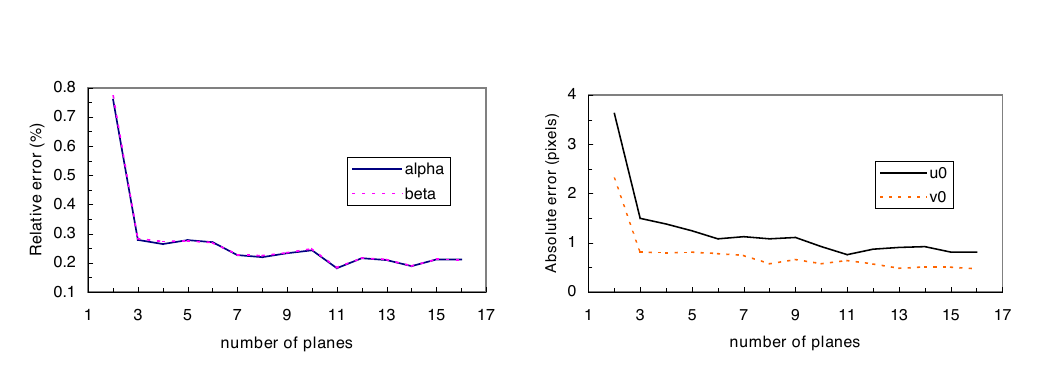
\includegraphics[width=0.92\linewidth]{figure2_num_images}
    \caption{模型平面图像数量对应的误差。}
    \label{fig:simulation-number}
\end{figure}

随着图像数量增加，误差逐渐减小；从 \(2\) 幅图像增加到 \(3\) 幅图像时，误差下降尤其明显。

\paragraph{模型平面姿态的影响}

该实验考察模型平面相对于图像平面的姿态对性能的影响。实验使用 \(3\) 幅图像。平面初始时与图像平面平行，然后从均匀球面上随机选择旋转轴，并绕该轴旋转 \(\theta\) 角。投影图像点上加入均值为 \(0\)、标准差为 \(0.5\) 像素的高斯噪声。重复这一过程 \(100\) 次并计算平均误差，\(\theta\) 从 \(5^\circ\) 变化到 \(75^\circ\)，结果如图\ref{fig:simulation-orientation}所示。

\begin{figure}[htbp]
    \centering
    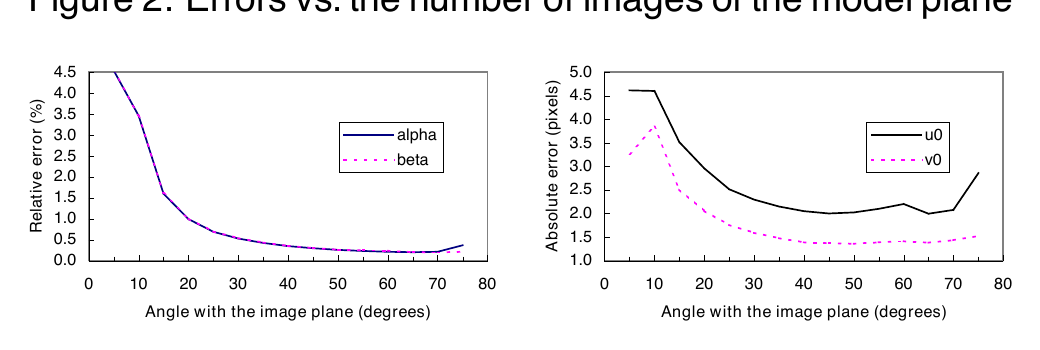
\includegraphics[width=0.92\linewidth,trim=0 0 0 9pt,clip]{figure3_orientation_angle}
    \caption{模型平面相对于图像平面的角度对应的误差。}
    \label{fig:simulation-orientation}
\end{figure}

当 \(\theta=5^\circ\) 时，由于各平面几乎相互平行，\(40\%\) 的试验失败（退化配置）；图\ref{fig:simulation-orientation}中的结果排除了这些失败试验。最佳性能似乎在约 \(45^\circ\) 的角度处取得。需要注意的是，在实际应用中，随着角度增大，透视缩短会使角点检测变得不够精确，但本实验没有考虑这一因素。

\subsection{真实数据}\label{subsec:real-data}

所提出的技术目前已在作者所在的视觉组和图形学组中常规使用。下面给出一个实例的结果。

待标定相机是一台配备 \(6\mathrm{mm}\) 镜头的商用 PULNiX CCD 相机，图像分辨率为 \(640\times480\)。模型平面包含 \(8\times8\) 个方格，因此共有 \(256\) 个角点；模板尺寸为 \(17\mathrm{cm}\times17\mathrm{cm}\)。拍摄了平面处于不同姿态下的 \(5\) 幅图像，如图\ref{fig:real-pattern}所示。可以观察到图像中存在明显的镜头畸变。角点通过拟合每个方格的直线，并取直线交点来检测。

\begin{figure}[htbp]
    \centering
    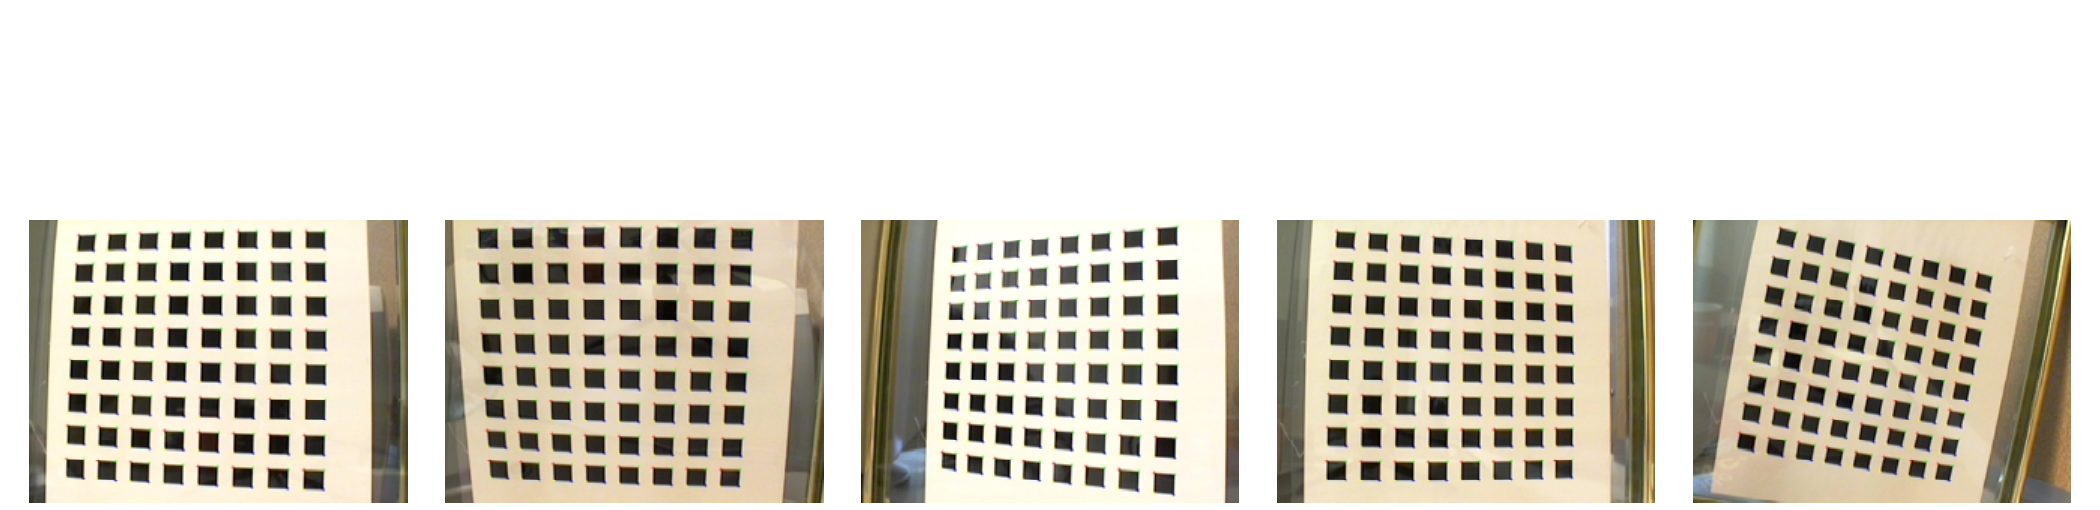
\includegraphics[width=0.98\linewidth]{figure4_five_model_images}
    \caption{模型平面的五幅图像及提取的角点；角点以十字标记表示，但标记过小，难以直接观察。}
    \label{fig:real-pattern}
\end{figure}

将标定算法分别应用于前 \(2\)、\(3\)、\(4\) 幅图像以及全部 \(5\) 幅图像，结果见表\ref{tab:real-results}。对于每种配置，表中给出三列结果：第一列（初始值）是闭式解的估计结果，第二列（最终值）是最大似然估计（MLE），第三列（\(\sigma\)）是估计的标准差，用于表示最终结果的不确定性。可以看出，闭式解是合理的；无论使用 \(2\)、\(3\)、\(4\) 还是 \(5\) 幅图像，最终估计值都非常一致。还可以看到，最终估计结果的不确定性随图像数量增加而减小。表\ref{tab:real-results}的最后一行 RMS 表示检测图像点与投影图像点之间距离的均方根，单位为像素；最大似然估计显著改善了这一指标。

\begin{table}[htbp]
    \centering
    \caption{使用 \(2\) 至 \(5\) 幅图像的真实数据标定结果。}
    \label{tab:real-results}
    \resizebox{\linewidth}{!}{%
    \begin{tabular}{c|ccc|ccc|ccc|ccc}
        \toprule
        \multicolumn{1}{c|}{图像数} & \multicolumn{3}{c|}{\(2\) 幅图像} & \multicolumn{3}{c|}{\(3\) 幅图像} & \multicolumn{3}{c|}{\(4\) 幅图像} & \multicolumn{3}{c}{\(5\) 幅图像}\\
        参数 & 初始 & 最终 & \(\sigma\) & 初始 & 最终 & \(\sigma\) & 初始 & 最终 & \(\sigma\) & 初始 & 最终 & \(\sigma\)\\
        \midrule
        \(\alpha\) & 825.59 & 830.47 & 4.74 & 917.65 & 830.80 & 2.06 & 876.62 & 831.81 & 1.56 & 877.16 & 832.50 & 1.41\\
        \(\beta\) & 825.26 & 830.24 & 4.85 & 920.53 & 830.69 & 2.10 & 876.22 & 831.82 & 1.55 & 876.80 & 832.53 & 1.38\\
        \(c\) & 0 & 0 & 0 & 2.2956 & 0.1676 & 0.109 & 0.0658 & 0.2867 & 0.095 & 0.1752 & 0.2045 & 0.078\\
        \(u_0\) & 295.79 & 307.03 & 1.37 & 277.09 & 305.77 & 1.45 & 301.31 & 304.53 & 0.86 & 301.04 & 303.96 & 0.71\\
        \(v_0\) & 217.69 & 206.55 & 0.93 & 223.36 & 206.42 & 1.00 & 220.06 & 206.79 & 0.78 & 220.41 & 206.56 & 0.66\\
        \(k_1\) & 0.161 & $-0.227$ & 0.006 & 0.128 & $-0.229$ & 0.006 & 0.145 & $-0.229$ & 0.005 & 0.136 & $-0.228$ & 0.003\\
        \(k_2\) & $-1.955$ & 0.194 & 0.032 & $-1.986$ & 0.196 & 0.034 & $-2.089$ & 0.195 & 0.028 & $-2.042$ & 0.190 & 0.025\\
        RMS & 0.761 & 0.295 & & 0.987 & 0.393 & & 0.927 & 0.361 & & 0.881 & 0.335 & \\
        \bottomrule
    \end{tabular}}
\end{table}

表\ref{tab:real-results}的 RMS 行原表仅列出初始值和最终值，没有给出 \(\sigma\)，因此对应单元格留空。

表\ref{tab:real-results}中 \(k_1\) 和 \(k_2\) 的闭式解与最大似然估计之间存在不一致，细心的读者可能会注意到这一点。原因在于，闭式解在假设不存在畸变的条件下估计相机内参数，预测得到的外侧点比检测点更靠近图像中心。随后进行的畸变估计试图使外侧点向外扩展并增大尺度，以减小误差；然而，这一过程中得到的畸变形状（正 \(k_1\)，称为枕形畸变）并不对应真实畸变（负 \(k_1\)，称为桶形畸变）。非线性细化（MLE）最终恢复了正确的畸变形状。估计得到的畸变参数可以用于校正原始图像中的畸变。

\begin{figure}[htbp]
    \centering
    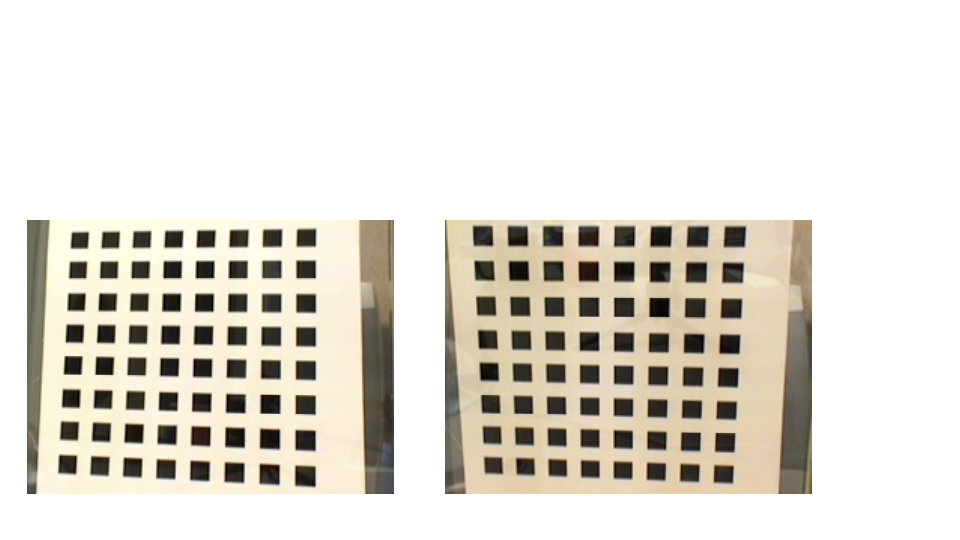
\includegraphics[width=0.72\linewidth]{figure5_corrected_images}
    \caption{径向畸变校正后的第一幅和第二幅图像。}
    \label{fig:real-corrected}
\end{figure}

图\ref{fig:real-corrected}显示了经过畸变校正的前两幅图像，应将其与图\ref{fig:real-pattern}中的前两幅图像进行比较。可以清楚地看到，原始图像中弯曲的图案被拉直了。

\paragraph{标定结果的变化}

上文表\ref{tab:real-results}给出了使用 \(2\) 至 \(5\) 幅图像时的标定结果；可以发现这些结果彼此非常一致。为进一步考察所提出算法的稳定性，将可用的 \(5\) 幅图像中所有由 \(4\) 幅图像组成的组合都用于标定，结果见表\ref{tab:quadruple-results}。例如，表中的第三列（1235）表示使用第 \(1\)、\(2\)、\(3\) 和 \(5\) 幅图像组成的组合。最后两列分别给出了 \(5\) 组结果的均值和样本标准差。所有参数的样本标准差都很小，这说明所提出的算法具有很好的稳定性。

\begin{table}[htbp]
    \centering
    \caption{所有四幅图像组合之间的标定结果变化。}
    \label{tab:quadruple-results}
    \resizebox{\linewidth}{!}{%
    \begin{tabular}{c|rrrrrrr}
        \toprule
        图像组合/参数 & (1234) & (1235) & (1245) & (1345) & (2345) & 均值 & 偏差\\
        \midrule
        \(\alpha\) & 831.81 & 832.09 & 837.53 & 829.69 & 833.14 & 832.85 & 2.90\\
        \(\beta\) & 831.82 & 832.10 & 837.53 & 829.91 & 833.11 & 832.90 & 2.84\\
        \(c\) & 0.2867 & 0.1069 & 0.0611 & 0.1363 & 0.1096 & 0.1401 & 0.086\\
        \(u_0\) & 304.53 & 304.32 & 304.57 & 303.95 & 303.53 & 304.18 & 0.44\\
        \(v_0\) & 206.79 & 206.23 & 207.30 & 207.16 & 206.33 & 206.76 & 0.48\\
        \(k_1\) & $-0.229$ & $-0.228$ & $-0.230$ & $-0.227$ & $-0.229$ & $-0.229$ & 0.001\\
        \(k_2\) & 0.195 & 0.191 & 0.193 & 0.179 & 0.190 & 0.190 & 0.006\\
        RMS & 0.361 & 0.357 & 0.262 & 0.358 & 0.334 & 0.334 & 0.04\\
        \bottomrule
    \end{tabular}}
\end{table}

偏斜参数 \(c\) 与 \(0\) 的差异并不显著，因为其变异系数 \(0.086/0.1401=0.6\) 较大。事实上，\(c=0.1401\)、\(\alpha=832.85\) 对应于图像两轴夹角为 \(89.99^\circ\)，这与 \(90^\circ\) 非常接近。我们还计算了每个四幅图像组合的纵横比 \(\alpha/\beta\)。纵横比的均值为 \(0.99995\)，样本标准差为 \(0.00012\)，因此它非常接近 \(1\)，即像素近似为正方形。

\paragraph{在基于图像的建模中的应用}

使用同一台已完成标定的相机拍摄了一个茶叶罐的两幅图像（见图\ref{fig:tea-tin-images}）。图像中主要可见茶叶罐的两个侧面。我们在每个侧面上手工选取了 \(8\) 个点匹配，并将此前开发的运动恢复结构软件应用于这 \(16\) 个点匹配，以建立茶叶罐的部分模型。重建模型采用 VRML 格式，图\ref{fig:tea-tin-model}给出了三个渲染视图。每个侧面上的重建点确实共面；计算得到的两个重建平面之间的夹角为 \(94.7^\circ\)。虽然没有真实值可供比较，但茶叶罐的两个侧面实际上确实几乎相互正交。

\begin{figure}[htbp]
    \centering
    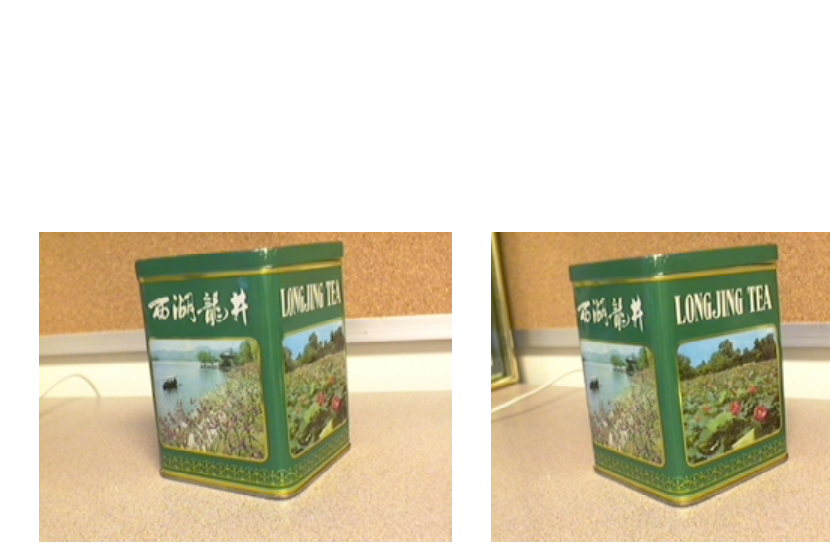
\includegraphics[width=0.72\linewidth]{figure6_tea_tin_images}
    \caption{茶叶罐的两幅图像。}
    \label{fig:tea-tin-images}
\end{figure}

\begin{figure}[htbp]
    \centering
    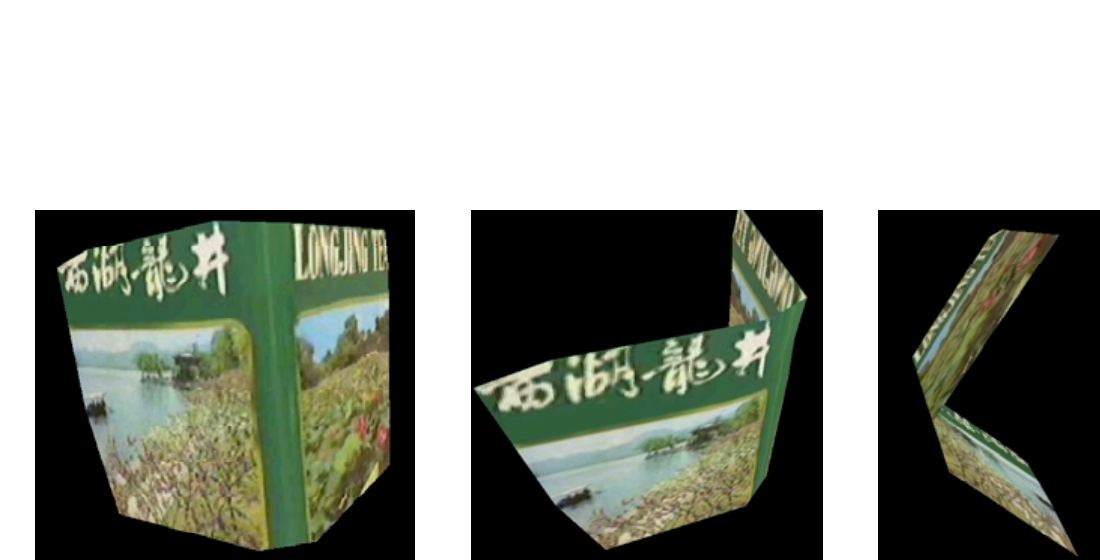
\includegraphics[width=0.86\linewidth]{figure7_reconstructed_views}
    \caption{重建茶叶罐的三个渲染视图。}
    \label{fig:tea-tin-model}
\end{figure}

包括全部真实数据、结果和软件在内的资料可从以下网页获得：
\begin{center}
\url{http://research.microsoft.com/~zhang/Calib/}。
\end{center}

% Section 6 translation from the user-provided paper.
\clearpage
\section{结论}\label{sec:conclusion}

本文提出了一种新的灵活技术，可以方便地完成相机标定。该技术只要求相机从少数几个（至少两个）不同方向观察一个平面模板。相机或平面模板均可移动，且不需要知道其运动。方法对径向镜头畸变进行了建模。所提出的流程由闭式解和随后基于最大似然准则的非线性细化组成。

我们使用计算机模拟和真实数据对所提出的技术进行了测试，并取得了非常好的结果。与需要使用两个或三个相互正交平面等昂贵设备的经典技术相比，所提出的技术具有显著的灵活性优势。

\section*{致谢}\label{sec:acknowledgment}

感谢 Brian Guenter 提供角点提取软件并进行了多次讨论，感谢 Bill Triggs 提供富有启发性的评论。感谢 Andrew Zisserman 使我注意到他的 CVPR98 工作~\cite{liebowitz1998metric}；该工作使用了相同的约束，但形式不同。感谢 Bill Triggs 和 Gideon Stein 建议开展关于模型不精确性的实验，该实验见技术报告~\cite{zhang1998flexible}。Anandan 和 Charles Loop 审阅了早期版本的英文。

\appendix
\section{模型平面与图像之间单应性的估计}

估计模型平面与其图像之间单应性的方法有很多。这里给出一种基于最大似然准则的技术。设 $\mathbf M_i$ 和 $\mathbf m_i$ 分别为模型点和图像点。理想情况下，它们应满足式~\eqref{eq:homography}。但在实际中，由于提取出的图像点含有噪声，这一关系并不严格成立。假设 $\mathbf m_i$ 受到均值为 0、协方差矩阵为 $\Lambda_{\mathbf m_i}$ 的高斯噪声干扰，则单应性矩阵 $\mathbf H$ 的最大似然估计通过最小化下列泛函得到：

\begin{equation*}
    \sum_i
    (\mathbf m_i-\widehat{\mathbf m}_i)^{\T}
    \Lambda_{\mathbf m_i}^{-1}
    (\mathbf m_i-\widehat{\mathbf m}_i),
\end{equation*}
其中
\begin{equation*}
    \widehat{\mathbf m}_i
    =\frac{1}{\overline{\mathbf h}_3^{\T}\widetilde{\mathbf M}_i}
    \begin{bmatrix}
        \overline{\mathbf h}_1^{\T}\widetilde{\mathbf M}_i\\
        \overline{\mathbf h}_2^{\T}\widetilde{\mathbf M}_i
    \end{bmatrix},
\end{equation*}
其中 $\overline{\mathbf h}_i$ 是 $\mathbf H$ 的第 $i$ 行。

在实践中，我们简单地对所有 $i$ 假设 $\Lambda_{\mathbf m_i}=\sigma^2\mathbf I$。如果各点是按照相同的过程彼此独立地提取的，这一假设是合理的。在这种情况下，上述问题变为非线性最小二乘问题，即
\begin{equation*}
    \min_{\mathbf H}\sum_i
    \left\lVert\mathbf m_i-\widehat{\mathbf m}_i\right\rVert^2.
\end{equation*}
非线性最小化采用 Minpack~\cite{more1977levenberg} 中实现的 Levenberg--Marquardt 算法完成。这需要一个初始猜测值，而该初始值可以如下获得。

令
\begin{equation*}
    \mathbf x=
    \begin{bmatrix}
        \overline{\mathbf h}_1^{\T} &
        \overline{\mathbf h}_2^{\T} &
        \overline{\mathbf h}_3^{\T}
    \end{bmatrix}^{\T}.
\end{equation*}
则式~\eqref{eq:homography} 可以改写为
\begin{equation*}
    \begin{bmatrix}
        \widetilde{\mathbf M}^{\T} & \mathbf 0^{\T} & -u\widetilde{\mathbf M}^{\T}\\
        \mathbf 0^{\T} & \widetilde{\mathbf M}^{\T} & -v\widetilde{\mathbf M}^{\T}
    \end{bmatrix}\mathbf x=\mathbf 0.
\end{equation*}
当给定 $n$ 个点时，就有 $n$ 个上述方程，它们可以写成矩阵方程 $\mathbf L\mathbf x=\mathbf 0$，其中 $\mathbf L$ 是一个 $2n\times9$ 矩阵。由于 $\mathbf x$ 只定义到一个尺度因子，众所周知，其解是与最小奇异值对应的 $\mathbf L$ 的右奇异向量（或者等价地，是与最小特征值对应的 $\mathbf L^{\T}\mathbf L$ 的特征向量）。

在 $\mathbf L$ 中，有些元素恒为 1，有些以像素为单位，有些以世界坐标为单位，还有一些是二者的乘积。这使得 $\mathbf L$ 在数值上条件很差。在执行上述过程之前进行简单的数据归一化（例如采用文献~\cite{hartley1995defence} 提出的方法），可以获得好得多的结果。

\section{从矩阵 B 提取内参数}

如第 3.1 节所述，矩阵 $\mathbf B$ 的估计只确定到一个尺度因子，即
\begin{equation*}
    \mathbf B=\lambda\mathbf A^{-\T}\mathbf A^{-1},
\end{equation*}
其中 $\lambda$ 是任意尺度因子。由矩阵 $\mathbf B$ 唯一地提取内参数并不困难。

\begin{align*}
    v_0
    &=\frac{B_{12}B_{13}-B_{11}B_{23}}
            {B_{11}B_{22}-B_{12}^{2}},\\
    \lambda
    &=B_{33}-\frac{B_{13}^{2}+v_0(B_{12}B_{13}-B_{11}B_{23})}
                         {B_{11}},\\
    \alpha&=\sqrt{\frac{\lambda}{B_{11}}},\\
    \beta&=\sqrt{\frac{\lambda B_{11}}
                         {B_{11}B_{22}-B_{12}^{2}}},\\
    c&=-\frac{B_{12}\alpha^{2}\beta}{\lambda},\\
    u_0&=\frac{cv_0}{\alpha}-\frac{B_{13}\alpha^{2}}{\lambda}.
\end{align*}

\section{用旋转矩阵逼近 3×3 矩阵}

本节所讨论的问题是求解一个最佳旋转矩阵 $\mathbf R$，以逼近给定的 $3\times3$ 矩阵 $\mathbf Q$。这里的“最佳”是指使差值 $\mathbf R-\mathbf Q$ 的 Frobenius 范数最小。相关解法可参见我们的技术报告~\cite{zhang1998flexible}。


\nocite{*}
\bibliographystyle{IEEEtran}
\bibliography{references}

\end{document}
